\documentclass[final]{beamer}
\usepackage[T1]{fontenc}
\usepackage{lmodern}
\usepackage[size=custom,width=120,height=72,scale=1.0]{beamerposter}
\usetheme{gemini}
\usecolortheme{gemini}
\usepackage{graphicx}
\graphicspath{{figures/}} 
\usepackage{booktabs}
\usepackage{tikz}
\usepackage{pgfplots}
\usepackage{csquotes}
\usepackage[
backend=biber,
style=numeric,
citestyle=numeric
]{biblatex}
\addbibresource{biblio.bib}

\usepackage[font=small,labelfont=bf]{caption} 

\newcommand{\compresslist}{
  \setlength{\itemsep}{1pt}
  \setlength{\parskip}{0pt}
  \setlength{\parsep}{0pt}}

\newcommand{\bfSigma}{\mbox{\boldmath$\Sigma$}}
\newcommand{\bfLambda}{\mbox{\boldmath$\Lambda$}}
\DeclareMathOperator*{\argmax}{\arg\!\max}
% ====================
% Lengths
% ====================

% If you have N columns, choose \sepwidth and \colwidth such that
% (N+1)*\sepwidth + N*\colwidth = \paperwidth
\newlength{\sepwidth}
\newlength{\colwidth}
\setlength{\sepwidth}{0.025\paperwidth}
\setlength{\colwidth}{0.3\paperwidth}

\newcommand{\separatorcolumn}{\begin{column}{\sepwidth}\end{column}}

% ====================
% Title
% ====================

\title{Some fancy title: followed by some more text}

\author{Alyssa P. Hacker \inst{1} \and Ben Bitdiddle \inst{2} \and Lem E. Tweakit \inst{2}}

\institute[shortinst]{\inst{1} Some Institute \samelineand \inst{2} Another Institute}

% ====================
% Body
% ====================

\begin{document}

\begin{frame}[t]
\begin{columns}[t]
\separatorcolumn

\begin{column}{\colwidth}

\begin{block}{Introduction}
Recurrent neural networks (RNN) constitute a family of neural network architectures
specialized to process sequential data. They do so by leveraging the simple idea
of sharing parameters across the model\cite{deeplearning}. They have been used in diverse domains for
generating sequences such as music and text. They can be trained by processing
real data sequences one step at a time and predicting what comes next.
In practice, early RNNs designs are unable to store information about far past
inputs. This fact diminishes their efficiency at modeling long structure. If
the network's predictions are based only on the last few inputs, which are
themselves predicted by the networks, then it has less chance to recover from
past mistakes. The solution to this problem seems to be a better memory and
especially a long-term memory for the network. 

Long Short-Term Memory (LSTM) are RNN designed to solve this problem. They are
better at storing informations than standard RNNs. It is important to note that
LSTM gives state-of-the-art results in a variety of sequence processing tasks.
This is the main reason why we decided to implement a LSTM for our text
generation project. We worked on 4 differents dataset: Harry Potter's books,
Lord of the ring's books, random quotes and a text from Shakespeare. 
\end{block}

\begin{block}{RNN structure} 
RNN comes from the following question: is there a neural network that depends
on the full previous context that would model: \begin{align*}
    P(o_1, \dots , o_T) = \prod_{t = 1}^T P(o_t | \hspace{0.05in} o_1, \ldots o_{t-1})
\end{align*}

They are feedforward neural networks with the addition of time dependency in
the model by introducing edges that span the adjacent time steps in the
network. At a given time, the nodes with recurrent edges receive input from the
current data and from the output of the hidden layer in the previous state, see
figure below. Thus, an input at time $t$ can influence the output at time $t + \delta$.
\begin{center}
    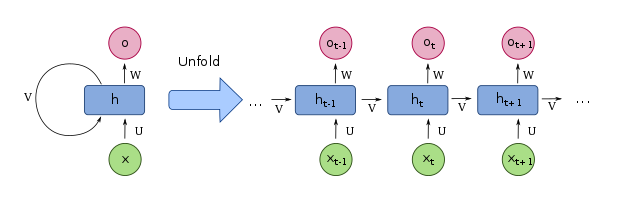
\includegraphics[width = 0.9\linewidth]{RNN.png}
\end{center}
\end{block}



\end{column}

\separatorcolumn

\begin{column}{\colwidth}

\begin{block}{RNN parameter udpates and vanishing-exploding gradient}
\begin{align*}
    &h_t = \sigma(U x_t + V h_{(t-1)} + b_h)\text{,}\\
    &o_t = \text{softmax}(W h_t + b_o)
\end{align*}

Here, $ U$, $V$ and $W$ are weights matrix. The vectors $b$ are bias
parameters. Learning with RNN is challenging due to dependencies between long
time steps. Consider the gradient with respect to $h_t$ of $o_{t + \delta}$.
How does it vary with $\delta$? Following the graph above and applying the
chain rule we can see that
\begin{equation*}
  \nabla_{h_t} o_{t + \delta} = \left( \prod_{k = t+1}^{t+\delta} V^T
  \text{diag}(1 - h^2_k) \right)\nabla_{h_{t + \delta}}o_{t + \delta}.
\end{equation*}

Thus, as $\delta$ grows, the gradient grows exponentially with $V$. If $V$ is
small or large than the gradient will either vanish or explode. This problem is
well known. Solutions exist, which brings us to present the LSTM.

\end{block}

  \begin{block}{Fusce aliquam magna velit}

    Et rutrum ex euismod vel. Pellentesque ultricies, velit in fermentum
    vestibulum, lectus nisi pretium nibh, sit amet aliquam lectus augue vel
    velit. Suspendisse rhoncus massa porttitor augue feugiat molestie. Sed
    molestie ut orci nec malesuada. Sed ultricies feugiat est fringilla
    posuere.

    \begin{figure}
      \centering
      \begin{tikzpicture}
        \begin{axis}[
            scale only axis,
            no markers,
            domain=0:2*pi,
            samples=100,
            axis lines=center,
            axis line style={-},
            ticks=none]
          \addplot[red] {sin(deg(x))};
          \addplot[blue] {cos(deg(x))};
        \end{axis}
      \end{tikzpicture}
      \caption{Another figure caption.}
    \end{figure}

  \end{block}

  \begin{block}{Nam cursus consequat egestas}

    Nulla eget sem quam. Ut aliquam volutpat nisi vestibulum convallis. Nunc a
    lectus et eros facilisis hendrerit eu non urna. Interdum et malesuada fames
    ac ante \textit{ipsum primis} in faucibus. Etiam sit amet velit eget sem
    euismod tristique. Praesent enim erat, porta vel mattis sed, pharetra sed
    ipsum. Morbi commodo condimentum massa, \textit{tempus venenatis} massa
    hendrerit quis. Maecenas sed porta est. Praesent mollis interdum lectus,
    sit amet sollicitudin risus tincidunt non.

    Etiam sit amet tempus lorem, aliquet condimentum velit. Donec et nibh
    consequat, sagittis ex eget, dictum orci. Etiam quis semper ante. Ut eu
    mauris purus. Proin nec consectetur ligula. Mauris pretium molestie
    ullamcorper. Integer nisi neque, aliquet et odio non, sagittis porta justo.

    \begin{itemize}
      \item \textbf{Sed consequat} id ante vel efficitur. Praesent congue massa
        sed est scelerisque, elementum mollis augue iaculis.
        \begin{itemize}
          \item In sed est finibus, vulputate
            nunc gravida, pulvinar lorem. In maximus nunc dolor, sed auctor eros
            porttitor quis.
          \item Fusce ornare dignissim nisi. Nam sit amet risus vel lacus
            tempor tincidunt eu a arcu.
          \item Donec rhoncus vestibulum erat, quis aliquam leo
            gravida egestas.
        \end{itemize}
      \item \textbf{Sed luctus, elit sit amet} dictum maximus, diam dolor
        faucibus purus, sed lobortis justo erat id turpis.
      \item \textbf{Pellentesque facilisis dolor in leo} bibendum congue.
        Maecenas congue finibus justo, vitae eleifend urna facilisis at.
    \end{itemize}

  \end{block}

\end{column}

\separatorcolumn

\begin{column}{\colwidth}

  \begin{block}{A block containing some math}

    Nullam non est elit. In eu ornare justo. Maecenas porttitor sodales lacus,
    ut cursus augue sodales ac.

    $$
    \int_{-\infty}^{\infty} e^{-x^2}\,dx = \sqrt{\pi}
    $$

    Interdum et malesuada fames $\{1, 4, 9, \ldots\}$ ac ante ipsum primis in
    faucibus. Cras eleifend dolor eu nulla suscipit suscipit. Sed lobortis non
    felis id vulputate.

    \heading{A heading inside a block}

    Praesent consectetur mi $x^2 + y^2$ metus, nec vestibulum justo viverra
    nec. Proin eget nulla pretium, egestas magna aliquam, mollis neque. Vivamus
    dictum $\mathbf{u}^\intercal\mathbf{v}$ sagittis odio, vel porta erat
    congue sed. Maecenas ut dolor quis arcu auctor porttitor.

    \heading{Another heading inside a block}

    Sed augue erat, scelerisque a purus ultricies, placerat porttitor neque.
    Donec $P(y \mid x)$ fermentum consectetur $\nabla_x P(y \mid x)$ sapien
    sagittis egestas. Duis eget leo euismod nunc viverra imperdiet nec id
    justo.

  \end{block}

  \begin{block}{Nullam vel erat at velit convallis laoreet}

    Class aptent taciti sociosqu ad litora torquent per conubia nostra, per
    inceptos himenaeos. Phasellus libero enim, gravida sed erat sit amet,
    scelerisque congue diam. Fusce dapibus dui ut augue pulvinar iaculis.

    \begin{table}
      \centering
      \begin{tabular}{l r r c}
        \toprule
        \textbf{First column} & \textbf{Second column} & \textbf{Third column} & \textbf{Fourth} \\
        \midrule
        Foo & 13.37 & 384,394 & $\alpha$ \\
        Bar & 2.17 & 1,392 & $\beta$ \\
        Baz & 3.14 & 83,742 & $\delta$ \\
        Qux & 7.59 & 974 & $\gamma$ \\
        \bottomrule
      \end{tabular}
      \caption{A table caption.}
    \end{table}

    Donec quis posuere ligula. Nunc feugiat elit a mi malesuada consequat. Sed
    imperdiet augue ac nibh aliquet tristique. Aenean eu tortor vulputate,
    eleifend lorem in, dictum urna. Proin auctor ante in augue tincidunt
    tempor. Proin pellentesque vulputate odio, ac gravida nulla posuere
    efficitur. Aenean at velit vel dolor blandit molestie. Mauris laoreet
    commodo quam, non luctus nibh ullamcorper in. Class aptent taciti sociosqu
    ad litora torquent per conubia nostra, per inceptos himenaeos.

    Nulla varius finibus volutpat. Mauris molestie lorem tincidunt, iaculis
    libero at, gravida ante. Phasellus at felis eu neque suscipit suscipit.
    Integer ullamcorper, dui nec pretium ornare, urna dolor consequat libero,
    in feugiat elit lorem euismod lacus. Pellentesque sit amet dolor mollis,
    auctor urna non, tempus sem.

  \end{block}

  \begin{block}{References}


  \end{block}

\end{column}

\separatorcolumn
\end{columns}
\end{frame}

\end{document}
